
\documentclass[draft]{agujournal2019}
\usepackage{url} \usepackage{lineno}
\usepackage[inline]{trackchanges} \usepackage{soul}
\usepackage{amsmath}
\linenumbers

\draftfalse


\journalname{Water Resources Research}


\begin{document}



\graphicspath{{/Users/songshgeo/Documents/VSCode/WGRegimes_YRB_2020/figures}}
\title{Identifying regime transitions for water governance at a basin scale}









\authors{
      Shuang Song\affil{1},
      Shuai Wang\affil{1},
      Xutong Wu\affil{1},
      yongping Wei\affil{2},
      Graeme S. Cumming\affil{3},
      Yue Qin\affil{4},
      Xilin Wu\affil{5},
      Bojie Fu\affil{1,5}
}


\affiliation{1}{
      State Key Laboratory of Earth Surface Processes and Resource Ecology,
      Beijing Normal University,
      Beijing, 100875, Beijing, China.
}
\affiliation{2}{
      School of Earth and Environmental Sciences,
      The University of Queensland,
      Brisbane, 4067, QLD, Australia.
}
\affiliation{3}{
      ARC Centre of Excellence for Coral Reef Studies,
      James Cook University,
      Townsville, 4811, QLD, Australia.
}
\affiliation{4}{
      College of Environmental Sciences and Engineering,
      Peking University,
      Beijing, 100875, Beijing, China.
}
\affiliation{5}{
      State Key Laboratory of Urban and Regional Ecology,
      Research Center for Eco-Environmental Sciences,
      Chinese Academy of Sciences,
      Beijing, 100875, Beijing, China.
}





\correspondingauthor{Shuai Wang}{shuaiwang@bnu.edu.cn}





\begin{keypoints}
\item We developed an Integrated Water Governance Index (IWGI) to detect regime shifts in water governance.
\item We interpret how water governance shifts within a rapidly-changing large river basin.
\item We developed an approach to analyzing intertwines of water governance, hydrosocial transition, and human-water relationships.
\end{keypoints}




\begin{abstract}
Water governance determine ``who gets water, when, and how'' in most large river basins.
Shifts in water governance regimes from natural to social-ecological or ``hydrosocial'' carry profound implications for human wellbeing; identifying regime changes in water governance is critical to navigating social-ecological transitions and guiding sustainability.
We characterized water governance along with the three main aspects - stress, purpose, and allocation - to develop a quantitative Integrated Water Governance Index (IWGI) at a basin scale.
Applying the IWGI to the rapidly-changing Yellow River Basin (YRB) in China clarifies shifts in water governance between massive supply, transformation governance, and adaptation-oriented regimes.
In the YRB, the underlying causes of regime shifts were increasing water supply and demand before the governance transformation and re-allocation and regulation after the change.
The IWGI offers a comprehensive and straightforward approach to linking water governance regimes to sustainability, providing valuable insights into hydrosocial transitions.
\end{abstract}

\section*{Plain Language Summary}
Missing governance means missing sustainability. However, the lack of a comprehensive but straightforward approach to identifying the changes in water governance presents a challenge for efforts to underpin it. Therefore, we choose indicators for the corresponding aspects (water stress, water services purpose, and water allocation) and combine them into an integrated water governance index (IWGI) to analyze long-term changes in a large river basin.


\section{Introduction}\label{sec1}
\label{Intro.}
Water, being ``at the centre of the planetary drama of the Anthropocene'', is essential not only for earth system processes but also in supporting development and human well-being
\cite{gleeson2020a,gleeson2020b}.
As an integral part of earth system governance, successful water governance requires a deep understanding of changes in the complex relationships between humans and water
\cite{ahlstrom2021,biermann2012,steffen2020}.
Human activities stemming from our reliance on water have profoundly modified the natural water cycle, resulting in rivers that are dominated by a hybrid of social and natural drivers
\cite{sivapalan2012,qin2014,abbott2019}.
Facing transitions from natural to human-dominated regimes, many big river basins worldwide (which are hot spots of civilization and economic growth) are urgently in need of more effective water governance
\cite{best2019,dibaldassarre2019}.

Water governance refers to the political, social, economic, and administrative systems that influence the use and management of water \cite{oecd2018, wang2017}, essentially about ``who gets water, when and how''\cite{lasswell2018}.
Therefore, the United Nations Development Programme (UNDP) has suggested that three core aspects of water use decided by water governance correspondingly: ``When and what water to use?'' (stress), ``How does water provide different services for human well-being?'' (purpose), and ``Who can use water equally and efficiently?'' (allocation)
\cite{undpwatergovernancefacility2016}.
First, water stress depends not only on climate (with increasing scarcity and uncertainty in many regions) but also on the increasingly insatiable demands from economic activities such as irrigation and industry; water storage can resolve some but not all of these issues
\cite{qin2019,wada2014,huang2021}.
Second, the purpose of how water services human well-being is to consider trade-offs between consumptive uses (e.g., drinking and food production) and non-consumptive uses (e.g., energy production)
\cite{liu2017,florke2018,jaeger2019}.
Third, the allocation of water across the whole basin is not only decided by regionally socio-economic and environmental context but also influenced by systematic regulation
\cite{schmandt2021,speed2013}.
Since the transition to a human-dominated regime induced substantive changes in the three interwind aspects (stress, purpose, and allocation), considering them seperately can lead to systematic failure in water governance.

A first critical step in understanding the successes and failures of water governance is to identify the different regimes that underpin it \cite{kjellen2015, grafton2013}.
Regimes of water governance arise within linked human-water systems (based on management, institutions, and exploitation) to create local equilibria in social-ecological structures and functions
\cite{falkenmark2021,bressers2013,loch2020}.
For example, under a human-dominated regime, reservoirs make water stress easier to be alleviated because of flexibility; growing energy and industrial demands make water services purposes lopsided to non-provisioning sectors; conveyance systems make water allocation more planned (Figure~\ref{fig:framework}~A)
However, the lack of a comprehensive but straightforward approach to identifying changes in water governance regimes represents a challenge for efforts to enhance the sustainability of water resource use.
Filling this gap, which is the aim of this paper, is essential for the appropriate alignment of human and water systems.


\begin{figure*}[!ht]
	\centering
	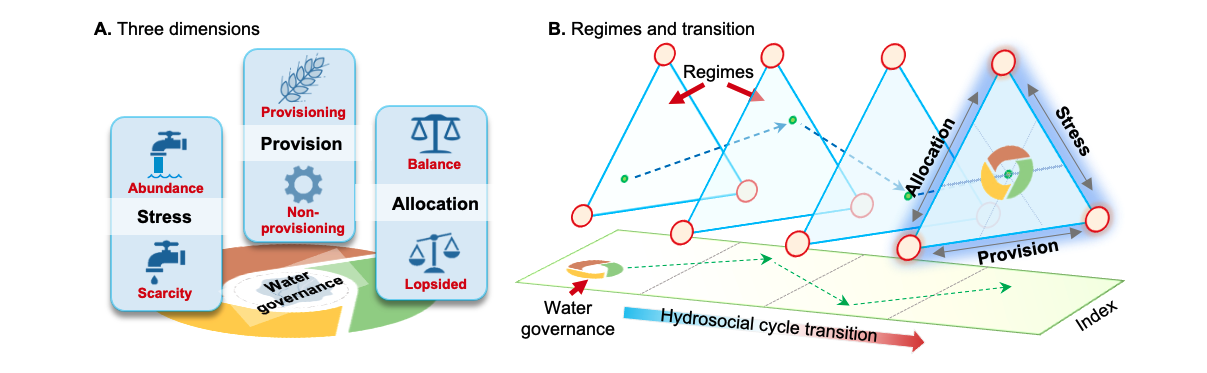
\includegraphics[width=0.9\textwidth]{main/framework.png}
	\caption{
		Identifying the water governance regimes in transitions of a hydrosocial cycle with an integrated water governance index (IWGI). Water stress (S), purposes of water services (P), and water allocation (A) are three aspects to be considered (\textbf{A.}). Along with hydrosocial-cycle transitions, a human-dominated regime influences these aspects of water governance. For example, the construction of reservoirs (1) aims to alleviate water stress; growth of energy and industry (2); water-lead intensive agriculture (3); conveyance system (4) controls water allocation.
		Therefore, the methodology is to combine three aspects' corresponding indicators, and then an abrupt change of the IWGI can indicate a regime shift in water governance (\textbf{B.}).
	}
	\label{fig:framework}
\end{figure*}


The Yellow River Basin (YRB), which contains the fifth-largest and most sediment-rich river in the world, needs integrated water governance because of geological and human history
\cite{mostern2021,best2019}.
Since the 1960s, governance practices such as reservoirs, levees, and conservation measures have contained the issues troubled by thousands of years of high sediment loads
\cite{wang2016e,song2020a}.
However, new challenges such as decreased streamflows and water depletions occurred in more recent times, leading to water use regulation and water transfer across basins -different focused water governance tactic
\cite{wang2019c}.
Today, it is still impossible to completely solve water stress, trade-offs between ecosystem services, or lopsided development in different regions in the YRB to the satisfaction of all actors
\cite{wohlfart2016a}.
Governance challenges induced by environmental, economic, social, and political factors have resulted in YRB being among the most intensively-governed large river basins worldwide \cite{nickum2021}.
Identifying regime shifts in water governance within the YRB can thus provide crucial insights into rapidly-changing big river basins and how governance may respond to meeting challenges to their sustainability.

Here, we depict the three aspects of water governance (stress, purpose and allocation) with corresponding indicators (see methods) and thus develop an Integrated Water Governance Index (IWGI) by equally weighting them, to indicate results from water governance (see Figure~\ref{fig:framework}~B).
Then, by applying the index to a typical rapid-changing big river basin (the YRB), we show how IWGI helps detect and describe complicated water governance regimes comprehensively but straightforwardly.
Following synthetic analyses of the changes in water demand, supply, economic outcomes, and institutions, we interpret the leading causes of the regime shifts.
Finally, we propose a general regime transition schema that offers a practical guideline for a coordinated approach to exploring the challenges faced by big river basin governance.

\section{Materials and Methods}\label{sec11}


To develop a comprehensive and straightforward approach to identifying water governance regimes. First, we constructed the Integrated Water Governance Index (IWGI) based on three aspects (Stress, Purpose, and Allocation, see Figure~\ref{fig:framework}). Then, we analyzed the changes in the IWGI from 1965 to 2013 using change point detection methods. The normalized Indicator for each dimension affects the IWGI by changing trends and contributions.

\subsection{Integrated Water Governance Index (IWGI)}

As shown in the framework Figure~\ref{fig:framework}, the IWGI combines the three aspects (Stress, Purpose, and Allocation) of water governance. Each dimension keeps two directions, and we assumed the hydrosocial cycle aligns with one of them, respectively:
	\begin{equation}
		Transformation \propto S*P*A
	\end{equation}

	We selected an indicator ($I_x$, $x=S$, $P$, or $A$, corresponding to stress, purpose, and allocation, respectively) to quantify the aspects effectively. Then, the above equation was transformed into a natural logarithm to facilitate calculation:
	\begin{equation}
		Transformation \propto \ln(I_S) + \ln(I_P) + \ln(I_A)
	\end{equation}

	Then, the Integrated Water Governance Index (IWGI) is an average of the normalized indicators $I'_x$:
	\begin{equation}
		IWGI = (I'_S + I'_P + I'_A) / 3
	\end{equation}

	where:
	\begin{equation}
		I'_x = (I_x - I_{x, \min}) / (I_{x, \max} - I_{x, \min})
	\end{equation}

	\subsubsection*{Indicator of stress}
	We used the scarcity-flexibility-variability (SFV) water stress index proposed in Qin et al., (2019) to evaluate water stress~\cite{qin2019}. This metric considers management measures (such as the construction of reservoirs) and the impact of changes in water use structure on the evaluation of water scarcity. Based on the hydrological and economic context of YRB, four second-level regions are divided (Source Region, Upper Region, Middle Region, and Lower Region, see \textit{Supporting Information S1}). For the whole YRB, the indicator of water stress $I_S$ is the average of all regions' SFV-index:
	\begin{equation}
		I_S = \frac{1}{4} * \sum_{i=1}^4 SFV_{i}
	\end{equation}

	Where $SFV_i$ is the SFV-index for region $i$, and the detailed calculation of $SFV_i$ can be found in the \textit{Supporting Information S2}.

	\subsubsection*{Indicator of purpose}
	To quantify purpose $I_P$, we used Non-Provisioning purpose Shares (NPS) of water use as an indicator. While provisioning purpose water use ($WU_{pro}$) includes domestic, irrigated, and livestock water uses, non-provisioning purpose water use ($WU_{non-pro}$) includes industrial and urban services water uses. We calculated the NPS as:
	\begin{equation}
		NPS = \frac{WU_{pro}}{WU_{pro} + WU_{non-pro}}
	\end{equation}

	In this study, we consider livestock water use, rural and urban domestic water use, and agricultural water use as provisioning water because they directly service for survival. Others are non-provisioning: services and industrial water use because they mainly service the economy.

	\subsubsection*{Indicator of allocations}
	To describe allocations $I_A$, we designed an indicator based on entropy, called Allocation Entropy Metric (AEM), which measures the degree of evenness in water allocation:

	\begin{equation}
		I_A = CEM = \sum_{i=1}^N - \log(p_{i}) * p_{i}
	\end{equation}

	where $p_{i}$ is the water proportion of region $i$ to the whole basin (here, $N=4$ considering divided regions in the YRB, see \textit{Supporting Information S1}).

	\subsection{Change points detection}
		With no assumptions about the distribution of the data, we applied the Pettitt (1979) approach of change-point detection to detect a single change-point in hydrological time series with continuous data~\cite{pettitt1979}.
		It tests $H0$: The variables follow one or more distributions with the exact location parameter (no change) against the alternative: a change point exists.
		Mathematically, when a sequence of random variables is divided into two segments represented by $\mathrm{x}_{1}, \mathrm{x}_{1}, \ldots, x_{t_{0}}$ and $x_{t_{0}+1}, x_{t_{0}+2}, \ldots, x_{T}$, if each segment has a common distribution function, i.e., $F_1(x)$, $F_2(x)$ and $F_1(x) \neq F_2(x)$, then the change point is identified at $t_0$. To achieve the identification of change point, a statistical index $U_{t,T}$ is defined as follows:

		\begin{equation}
			U_{t, T} = \sum_{i=1}^t\sum_{j=t+1}^T sgn(X_i - X_j), 1 \leq t < T
		\end{equation}

		where:
		\begin{equation}
			\operatorname{sgn}(\theta)= \begin{cases}1 & \text { if } \theta>0 \\ 0 & \text { if } \theta=0 \\ -1 & \text { if } \theta<0\end{cases}
		\end{equation}

		The most probable change point $\tau$ is found where its value satisfies $K_{\tau} = \max|U_{t, T}|$ and the significance probability associated with value $K_{\tau}$ is approximately evaluated as:
		\begin{equation}
			p=2 \exp \left(\frac{-6 K_{\tau}^{2}}{T^{2}+T^{3}}\right)
		\end{equation}
		Given a certain significance level $\alpha$, if $p < \alpha$, we reject the null hypothesis and conclude that $x_{\tau}$ is a significant change point at level $\alpha$.

We used $\alpha = 0.001$ as the threshold level of the p-value, meaning that the probability of a statistically significant change-point judgment being valid was more than $99.9\%$. We divided the series into two at that point and analyzed each series separately until all significant change points were detected. Though two break points in the main text with $\alpha = 0.001$, the threshold from $0.0005$ to $0.05$ does not affect our results, and the breakpoints we identified are robust (see \\textit{Supporting Information} Figure~S3).

	\subsection{Datasets}
In order to calculate IWGI in the YRB, all the datasets we need are listed in the \textit{SI Appendix} Table~S1 with a detailed description in \textit{Supporting Information S3}.
 \section{Results}\label{sec2}
\subsection{Water governance regimes}\label{Res.1}

\begin{figure*}[ht!]
	\centering
	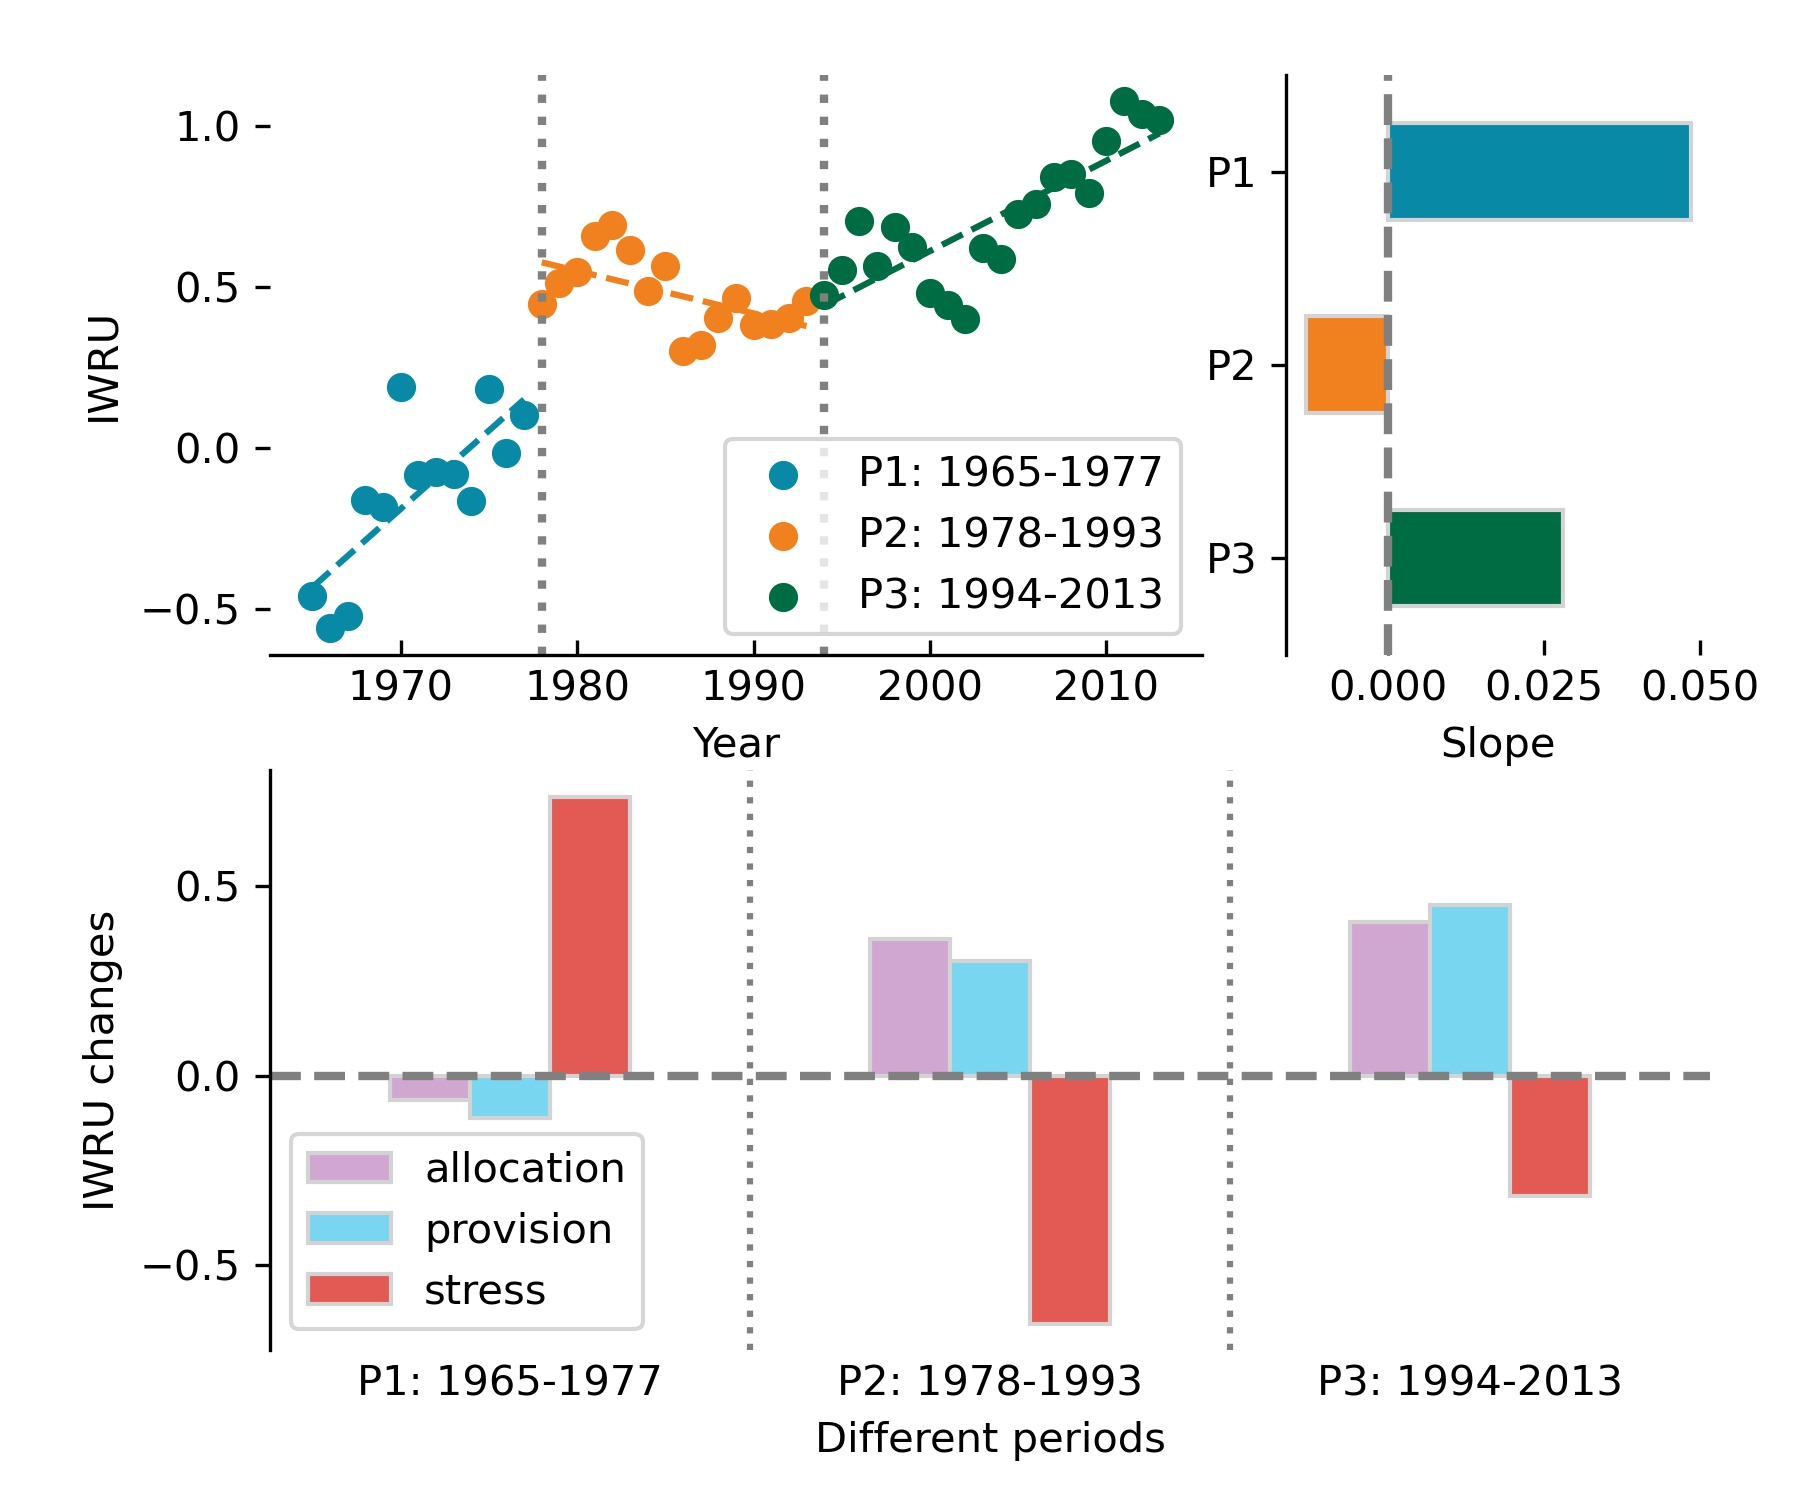
\includegraphics[width=0.9\linewidth]{main/index.jpg}
	\caption{Changes in the IWGI index and corresponding water governance regimes: P1: $1965 \sim 1978$, P2: $1979 \sim 2001$, and P3: $2002 \sim 2013$.
	\textbf{A,} detecting change points of IWGI and contributions from each indicator. Two significant change points ($p<0.01$) occurred in 1978 and 2001.
	\textbf{B,} correlation of trends between the IWGI and the indicators.
	\textbf{C,} across three indicators, changing components of the IWGI, whose directions shifts between different regimes.
	}\label{fig:IWGI}
\end{figure*}

Two significant breakpoints divide the changes in the IWGI into three periods, with different contributions from three aspects (Figure~\ref{fig:IWGI}A).
In the first period (P1, $1965 \sim 1978$), the IWGI decreased rapidly.
While the indicator of purpose and allocation contributed more to the IWGI ($49.45\%$ and $34.95\%$ on average, respectively), the remarkable downward trend correlates significantly ($p<0.01$) to the decreasing allocation and stress indicators (Figure~\ref{fig:IWGI}B).
In the second period (P2, $1979 \sim 2001$), the increasing stress indicator significantly ($p<0.01$) contributed to the upward IWGI, while the allocation and purpose indicators played negative roles in changing the IWGI.\
During the third period (P3, $1995 \sim 2013$), while the stress indicator kept its most prominent share in contributions ($57.11\%$ on average), the increased allocation indicator and decreased purpose indicator changed the regime.
Taken together, the overall features of the three aspects in different periods are relative to a directional change in the combination of three aspects (Figure~\ref{fig:IWGI}C).

\subsection{Causes of the regime shifts}\label{Res.2}

\begin{figure*}[th!]
	\centering
	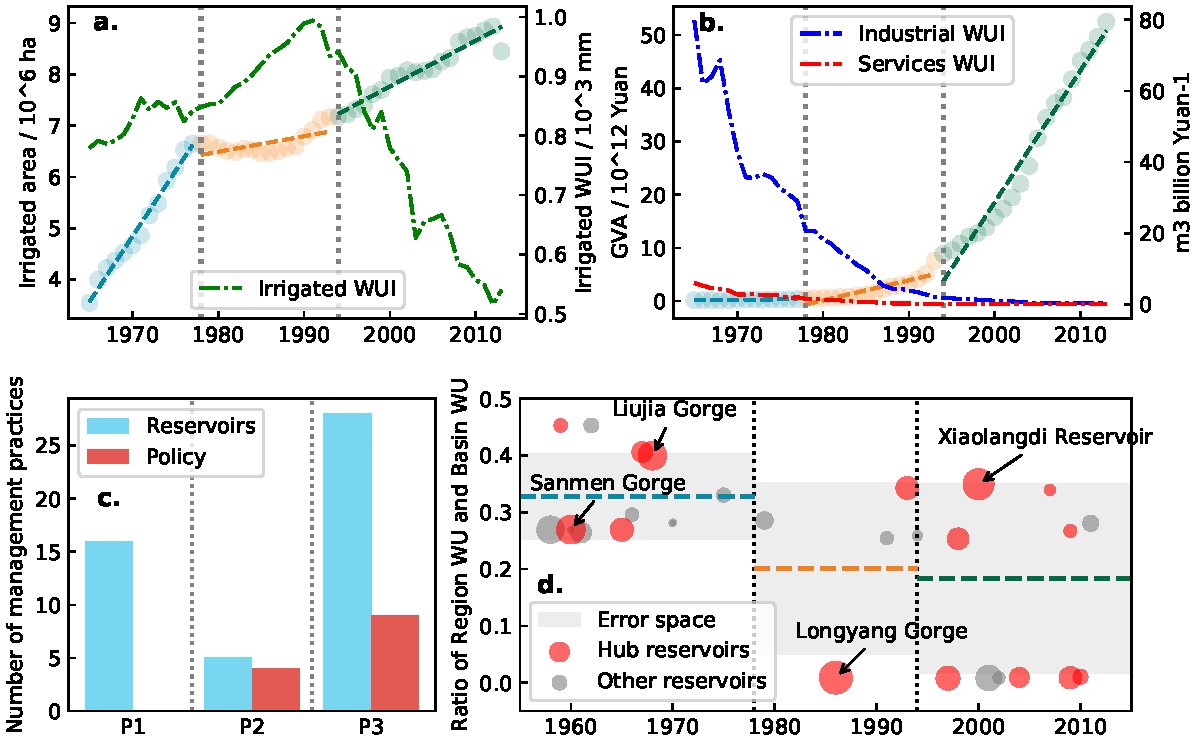
\includegraphics[width=0.9\linewidth]{main/causes.pdf}
	\caption{
		Causes of water governance regime shifts in the YRB.\
		\textbf{A.} Changes in the total irrigated area (orange line) and water use intensity ($WU/A$, water use divided by the irrigated area, the green dot line).
		\textbf{B.} Changes in gross values added (GVA) of industry and services (blue line) and their water use intensities ($WU/GVA$ WU divided by the GVA, the red dot line).
		\textbf{C.} Completed time of each new reservoir and their located region's water use (LWU) percentages as a proportion of the total basinal water use (BWU) at that time. Red circles denote the reservoirs mainly for managing and regulating the whole basin.
		The size of each circle indicates the magnitude of its water storage capacity.
		\textbf{D.} Social transformations (red triangles) and national-level governance policies (the circles, different colours denote signed by different state institutions, see \textit{Supporting Information} Table~S2). The light grey bars count official documents related to the YRB on a basinal scale (the Yellow River Events).
	}\label{fig:Causes}
\end{figure*}

The underlying causes of changes in the IWGI are different in the two regime shifts.
Changing water demands and supply were critical to the shift between P1 and P2.
As the dominant water demand during the P1, the area of irrigated agriculture in the YRB expanded rapidly at a rate of $0.25*10^6~ha/yr$ (Figure\ref{fig:Causes}~A), simultaneously supported by increasing supply through the construction of reservoirs (\textit{Supporting Information} Figure~S2). Ensuing the P2, however, the expansion of irrigated areas slowed down, and industry and services gradually took off (Figure\ref{fig:Causes}~A and B).
Then, the efficiency of water use changed obviously from P2 to P3.
Not only did irrigated areas continue to expand slowly during the P3 (Figure\ref{fig:Causes}~A), but industry and urban services also assumed a more vital economic role (represented by Gross Added Values, GVA) (Figure~\ref{fig:Causes}~B).
Because of increased efficiency, however, they both experienced significant declines in water use for a unit irrigated area or unit production (Figure~\ref{fig:Causes}~A and Figure~\ref{fig:Causes}~B).
As a result, the differences between sectors and regions in water use reduced while the total water stress steadily remained high during the P3 (Figure~\ref{fig:IWGI}A).

Environmental context, social transformation, and policies played roles in all three periods.
We calculated the ratios of regional and basinal water use for each reservoir (R/B ratio) (Figure~\ref{fig:Causes}C), with a higher ratio representing a potential role in water supply rather than basinal regulations.
Under the banner of ``conquering nature'' most of the reservoirs were built in regions with high water demands during the P1 (R/B ratios were significantly higher ($p<0.01$, see Figure~\ref{fig:Causes}C)).
Ensuing the P2, the number of new reservoirs decreased significantly and significantly increased basin policies rigorously controlled the allocation of water (Figure~\ref{fig:Causes}D, $p<0.01$ and \textit{Supporting Information} Figure~S2).
During the P3, authorities proposed more national-level water governance policies under the guidance of the national strategy ``environmental regulation'' (Figure~\ref{fig:Causes}D).
The regime shift from P1 to P2 is in line with the increasing water supply and demands; while driven by regulatory policies and efficiency enhancement under stable water stress from P2 to P3.


\section{Discussion}\label{sec12}

Water governance gradually becomes a national or international concern from a primarily local concern because large river basins are critical sources of ecosystem services, economic development, and human well-being~\cite{best2019,best2020}.
As tele-coupling raises additional water governance challenges in an increasingly tightly-connected world, regime shifts in water governance align with different human-water relationships~\cite{diaz2019}.
The process echoes how societies have been proposed to change governance practices by enhancing their adaptive capacity in the hydrosocial cycle, and the IWGI quantitatively identifies this transition~\cite{loch2020,turton1999}.
It is vital for scientists and decision-makers to recognize the changing governance challenges because models, institutions, engineering, and approaches developed under one regime are not necessarily applicable under a different regime~\cite{reyers2018}.

In the case of the YRB, our results show that there have been three distinct governance regimes; we named them: a massive supply regime (P1: $1965 \sim 1978$), a governance transforming command (P2: $1979 \sim 2001$), and an adaptation oriented regime (P3: $2002 \sim 2013$) (Figure~\ref{fig:IWGI}).
During the massive supply regime with lower water stress ($1965 \sim 1978$ in the YRB), water governance thus tended to boost water supply for services (mainly provisioning purposes then -livestock and crops) by constructing reservoirs and channels.
As the Chinese slogan ``man will conquer nature'' suggested then, however, the enhancement of water supply did not align with irreversible changes in the human-water relationship; it drastically increased water demand with little consideration for ecological conservation~\cite{zhou2020}.
The rapid expansion of irrigated farmland and water diversion facilities in the same decade brought the overburdened YRB close to a critical point, where increasing supply to meet demand was impractical~\cite{loch2020}.
Use of over $80\%$ of the surface water since 1972 has led to frequent river depletion, causing additional ecological issues such as wetland shrinkage and declines in biodiversity~\cite{wang2019c}.
In addition, since water stress also limited the growing industrial economy, the existing modes of water governance led to a social-ecological crisis~\cite{wohlfart2016a}.

The start of the governance transforming regime (P2: $1979 \sim 2001$) coincided with rising competition for water use after the ``reform and opening-up''.
The results from the YRB mirror those of the theoretical analysis: continuous increases in water demand when the basin's total supply is stable can follow substantial changes in governance regime and a rapid enhancement in overall social adaptive capacity~\cite{loch2020}.
As a pioneer in shifting governing institutions, the YRB triggered institutional changes during this regime. These include, for example, slowing the growth of irrigated acreage; leading water-saving infrastructure; creation of China's first water quota scheme, and the creation of a preliminary cross-boundary water transfer plan~\cite{wang2019a,long2020,nickum2021}.
Consequently, although water stress remained and increased (due to reducing streamflow and flexibility), the last depletion of the Yellow River in 1999 led to a climax in this transformation in water governance~\cite{wang2019a}.

The ensuing adaptation-oriented regime (P3: $2002 \sim 2013$) involved a significant societal shift in adapting to stable high water stress.
Socio-economic trade-offs between water-dependent regions and sectors played a more important role in this regime, so water governance had to achieve efficient water allocation while balancing different demands in the face of limited water supply~\cite{dalin2015,song2022}.
Widespread reconstruction of resources in different industries and regions led to calls for adaptation in water governance, using the urgent requirements of adjusting rigid quota shares from the previous regime as an example~\cite{wang2019a}.
Many national-level governance practices were proposed under the regime because the absence of such policies to support high-quality development became new a structural challenge for water governance~\cite{konar2019}.

In general, water governance of the YRB is among the most prominent example in the widespread transition to a hydrosocial cycle -``improving supply, transforming governance, and enhancing adaptation''.
With each dimension changing gradually, the emergence of different regimes drives water governance challenges at a basin-scale: these were primarily economic and environmental before the transformation, but social and policy-related towards the end (Figure~\ref{fig:summary})~\cite{singh2019,porcher2019}.
In an analogy at a global scale, the resource challenges, represented by water shortage and water supplying difficulties, are mainly faced by undeveloped and developing basins~\cite{allan2019,speed2013,liu2012a}.
Highly-controlled and developed basins (especially for transboundary rivers) must mainly resolve structural challenges, such as water disputes or lack of equity, and may be in urgent need of novel flexible, efficient sociopolitical governance structures~\cite{unep-dhi2016,mirumachi2015}.
Linking regime shifts to the governance challenges, the implementation of IWGI thus offers a comprehensive and straightforward way to interpret the intertwines between water governance and the hydrosocial transition.


\begin{figure*}[htbp!]
	\centering
	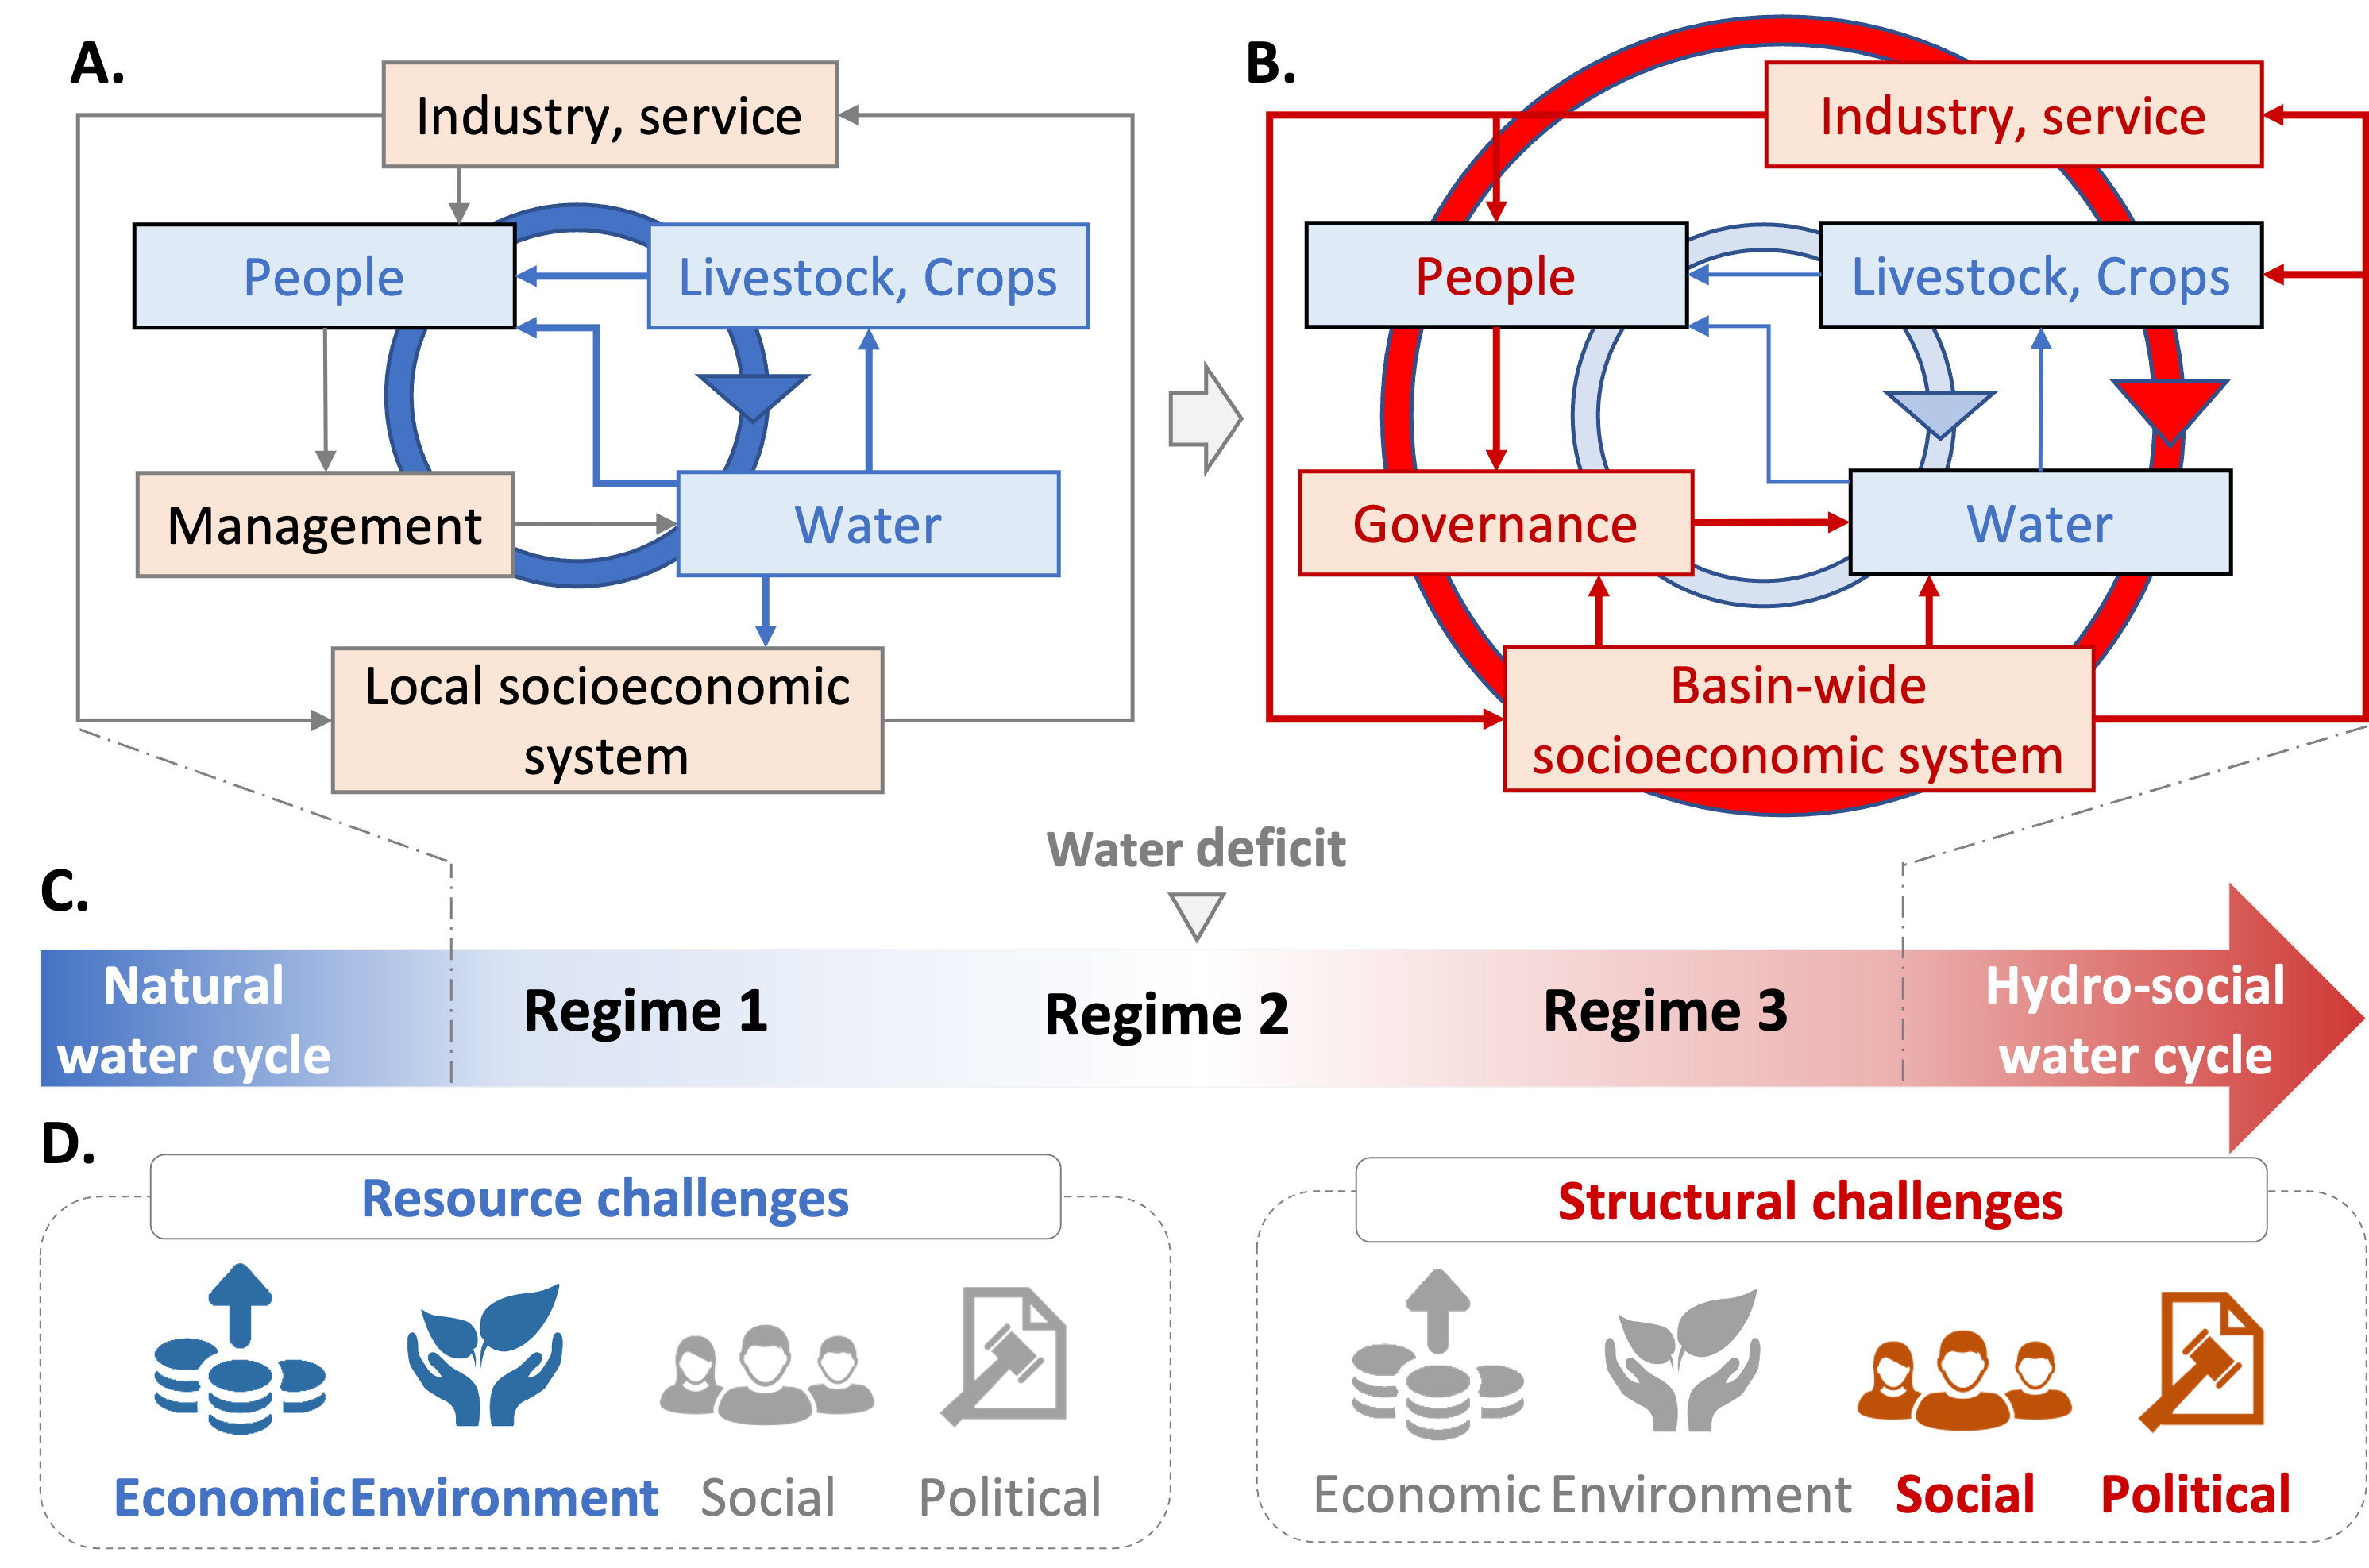
\includegraphics[width=0.8\linewidth]{main/transition.png}
	\caption{
		Transition schema in hydrosocial cycle and water governance regimes. The natural water cycle dominates blue pathways, while socio-economic feedback dominates red.
		\textbf{A.} As socio-economic systems develop, non-provisioning water demand increases; simultaneously, increased adaptive capacity by engineering allows people to manage water resources to alleviate water stress.
		\textbf{B.} With further human interventions, trade-offs between provisioning-purpose and non-provisioning water use become prominent; a basin-wide socio-economic system requires more organized water governance.
		Thus, \textbf{C. the hydrosocial water cycle transition} correlates with the water governance regime shifts. The transformation governance regime shift occurs following the water deficit, with the rapid growth of adaptive capacity.
		\textbf{D. Water governance challenges} Through the transitional regimes, water governance faces primarily economic and environmental challenges but social and policy challenges later.
	}\label{fig:summary}
\end{figure*}


One of the main limitations in the approach is the lack of long-term data worldwide, which means there is still a gap between comprehensively identifying and applying the IWGI more widely.
However, we propose that all water governance issues result in changing ``who gets water, when and how'', so monitoring water stress, purposes of water services, and water allocation patterns do help.
Choices of indicators for different aspects can be adapted according to available datasets; the connections between underlying components remain crucial in holistically understanding transitions in governance regimes.
In today's world, regime shifts from biophysical to hydrosocial control of water dynamics seem likely to become increasingly widespread; comprehensive strategies to address governance challenges will have to become the core of complex human-water systems~\cite{cumming2018,cumming2014,jaeger2019}.
Although river basins have shown improvements in water management technologies and water use efficiency, many are still approaching local, regional, and planetary boundaries where human-water systems may collapse~\cite{gleeson2020, wang-erlandsson2022}.
A deeper understanding of governance that incorporates ideas of non-linear regime shifts and transformations should help shift the focus of governance towards maintaining the resilience of the basin’s social-ecological system and improving its sustainability~\cite{falkenmark2019}.

\section{Conclusion}\label{sec13}
Focusing on ``who gets water, when and how'', three aspects of water governance change along with the hydrosocial cycle transition: water stress, water services purpose, and water allocation. We developed an Integrated Water Governance Index (IWGI) to detect regime shifts in water governance by integrating them. Applying the IWGI to a rapidly-changing large river basin (the Yellow River Basin, China), we interpret how water governance shifts between three regimes over half a century. Our approach quantitatively identifies the general schema for water governance regimes in the YRB, in line with previous theoretical analysis with a representative transition process. Linking regime shifts to the underlying causes, the implementation of IWGI offers a comprehensive and straightforward way to interpret changes in intertwines of water governance, hydrosocial transition, and human-water relationships.
























\section*{Open Research Section}
All the used datasets and access source are listed in the \textit{SI Appendix} Table~S1 with a detailed description in \textit{Supporting Information S3}.



\acknowledgments
Funding was provided by the National Natural Science Foundation of China (CN) (Grant Nos. NSFC 42041007).

\bibliography{../mybibtex.bib}






\end{document}
